\tikzstyle{format} = [draw, thin, fill=blue!20]
\tikzstyle{pblock} = [rectangle, draw, fill=blue!20, text width=6em, text centered, rounded corners, minimum height=0.4em]
\tikzstyle{mblock} = [rectangle, draw, fill=green!20, text width=6em, text centered, rounded corners, minimum height=0.4em]
\tikzstyle{bblock} = [rectangle, draw, fill=gray!20, text width=6em, text centered, rounded corners, minimum height=0.4em]
\tikzstyle{prblock} = [rectangle, draw, fill=red!20, text width=6em, text centered, rounded corners, minimum height=0.4em]
\tikzstyle{rblock} = [rectangle, draw, fill=black!50, text width=6em, text centered, rounded corners, minimum height=0.4em]
%\tikzstyle{block} = [rectangle, draw, fill=blue!20, text centered, rounded corners]
\tikzstyle{decision} = [diamond, draw, fill=blue!20, text width=4.5em, text badly centered, node distance=3cm, inner sep=0pt]
\tikzstyle{medium} = [ellipse, draw, thin, fill=green!20, minimum height=2.5em]
\tikzstyle{cloud} = [draw, ellipse,fill=red!20, node distance=3cm, minimum height=2em]
\tikzstyle{line} = [draw, -latex']
\tikzstyle{emptyblock} = [rectangle]
\tikzstyle{progblock} = [rectangle, draw, fill=yellow!20, text width=6em, text centered, minimum height=0.4em]

\begin{tikzpicture}[scale=0.7,transform shape,node distance=2.7cm]%[node distance = 3cm, scale=0.5]
    % Place nodes
    \node [pblock] (STEP) {
		     STEP file};
    \node [progblock, right of=STEP] (BOGUI) {
		     heronion};
    \node [mblock, right of=BOGUI] (surfmesh) {
		     surface mesh};
    \node [mblock, below of=surfmesh] (add) {
		     mesh, ...};
    \node [pblock, right of=surfmesh] (H5FED) {
		     H5FED};
    \node [pblock, above of=H5FED] (H5Part) {
		     H5Part};

  \node [progblock, above of=H5Part] (H5PartROOT) {
		     H5PartROOT};


    \node [pblock, below of=H5FED] (VTK) {
    		     VTK};
    \node [progblock, right of=H5FED] (OPAL) {
    		     OPAL};


% The disk
 \coordinate (mydisk1) at (13,-0.5);
 \coordinate (mydisk2) at (13.5,-0.5);
 \draw[fill=blue!60, fill opacity=0.5] (12,-0.5) to [controls=+(90:0.5) and +(90:0.5)] (14,-0.5);
 \draw[fill=blue!60, fill opacity=0.5] (12,-0.5) .. controls +(-90:0.5) and +(-90:0.5) .. (14,-0.5);
 \draw[fill=blue!60, fill opacity=0.5] (12,-0.5) .. controls +(-90:0.5) and +(-90:0.5) .. (14,-0.5) -- (14,-2) .. controls +(-90:0.5) and +(-90:0.5) .. (12,-2) -- (12,-0.5);
 \draw (13,-1.5) node {Disk};
   
		  
    % Draw edges
    \path [line] (STEP) -> (BOGUI);
    \path [line] (BOGUI) -> (surfmesh);
    \path [line,style=dashed, ->] (BOGUI) edge [out=-90, in=90] (add);
    \path [line] (surfmesh) -> (H5FED);
    \path [line,style=dashed, ->] (surfmesh) edge [out=-90, in=90] (VTK);
    %\path [->] (fifth) edge [out=-90, in=90] (distmesh);
    \path [<->] (H5FED) edge (OPAL);
    \path [line,style=dashed, ->] (H5FED) edge [out=90, in=180] node[right] {part of} (H5Part);
    \path [<->] (H5Part) edge [out=0, in=90] (OPAL);
    \path [<->] (OPAL) edge [out=0, in=90] (mydisk1);
    \path [<-] (H5PartROOT) edge [out=0, in=90] (mydisk2);	
    
   \node (pic1) at (3,3.5) { 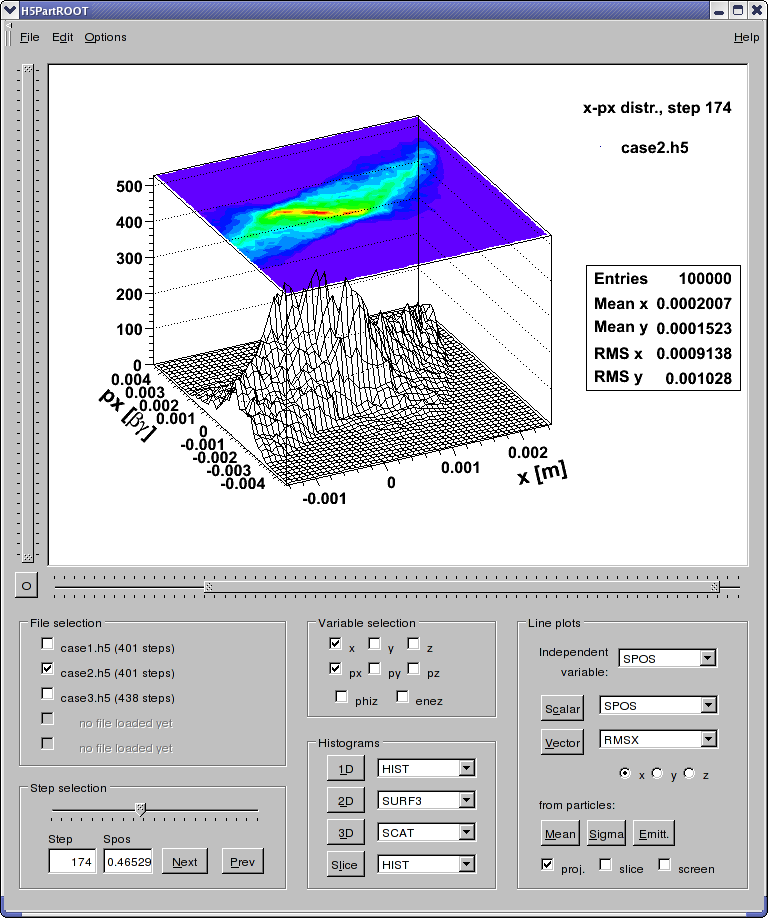
\includegraphics[width=0.35\linewidth]{figures/H5PartROOT}};
   \node (txtpic1) at (1,6.5) {\bf{H5PartROOT}};
    
    		
\end{tikzpicture}

%\begin{tikzpicture}
% \draw[fill=blue!60, fill opacity=0.5] (0,-0.5) to
%        [controls=+(90:0.5) and +(90:0.5)] (2,-0.5);
%    \draw[fill=blue!60, fill opacity=0.5] (0,-0.5) .. controls +(-90:0.5)
%    and +(-90:0.5) .. (2,-0.5);
%    \draw[fill=blue!60, fill opacity=0.5] (0,-0.5) .. controls +(-90:0.5)
%    and +(-90:0.5) .. (2,-0.5)
%        -- (2,-2) .. controls +(-90:0.5) and +(-90:0.5) .. (0,-2) -- (0,-0.5);
%\end{tikzpicture}



%\begin{tikzpicture}[overlay]
%	\path[->]<1-> (third) (fifth);
%	\path[->,red!40,thick]<2-> (second) edge [bend right] (fifth);
%\end{tikzpicture}
